\documentclass{article}

% Recommended, but optional, packages for figures and better typesetting:
\usepackage{microtype}
\usepackage{graphicx}
\usepackage{subfigure}
\usepackage{booktabs} % for professional tables

% hyperref makes hyperlinks in the resulting PDF.
% If your build breaks (sometimes temporarily if a hyperlink spans a page)
% please comment out the following usepackage line and replace
% \usepackage{icml2021} with \usepackage[nohyperref]{icml2021} above.
\usepackage{hyperref}

\usepackage{url}            % simple URL typesetting
\usepackage{booktabs}       % professional-quality tables
\usepackage{amsfonts}       % blackboard math symbols
\usepackage{nicefrac}       % compact symbols for 1/2, etc.
\usepackage{microtype}      % microtypography


\usepackage{amsmath}
\usepackage{bm}
\usepackage{bbm}
\usepackage{xcolor}
\usepackage{graphicx}
\usepackage{overpic}
\usepackage{wrapfig}

\usepackage{siunitx}
\sisetup{output-exponent-marker=\ensuremath{\mathrm{e}}}

% \DeclareMathOperator*{\cgrad}{grad}
\newcommand{\cgrad}{\operatorname{grad}}
\DeclareMathOperator*{\cdiv}{div}
\DeclareMathOperator*{\dd}{d}
\DeclareMathOperator*{\diag}{diag}
\DeclareMathOperator*{\vect}{vec}
\DeclareMathOperator*{\real}{Re}

\newcommand{\code}[1]{\texttt{#1}}
\newtheorem{prop}{Proposition}
\newtheorem{thm}{Theorem}
\newtheorem{lem}{Lemma}

\newcommand{\michael}[1]{{\color{red}\sf{[Michael: #1]}}}
\newcommand{\charles}[1]{{\color{blue}\sf{[Charles: #1]}}}

\newcommand{\fakesection}[1]{%
  \par\refstepcounter{section}% Increase section counter
  \sectionmark{#1}% Add section mark (header)
  \addcontentsline{toc}{section}{\protect\numberline{\thesection}#1}% Add section to ToC
  % Add more content here, if needed.
}

% Attempt to make hyperref and algorithmic work together better:
\newcommand{\theHalgorithm}{\arabic{algorithm}}

% Use the following line for the initial blind version submitted for review:
\usepackage{icml2021}

% If accepted, instead use the following line for the camera-ready submission:
% \usepackage[accepted]{icml2021}

% The \icmltitle you define below is probably too long as a header.
% Therefore, a short form for the running title is supplied here:
\icmltitlerunning{A Differential Geometry Perspective on Orthogonal Recurrent Models}

\begin{document}

\twocolumn[
\icmltitle{XXX TITLE}

% It is OKAY to include author information, even for blind
% submissions: the style file will automatically remove it for you
% unless you've provided the [accepted] option to the icml2021
% package.

% List of affiliations: The first argument should be a (short)
% identifier you will use later to specify author affiliations
% Academic affiliations should list Department, University, City, Region, Country
% Industry affiliations should list Company, City, Region, Country

% You can specify symbols, otherwise they are numbered in order.
% Ideally, you should not use this facility. Affiliations will be numbered
% in order of appearance and this is the preferred way.
\icmlsetsymbol{equal}{*}

\begin{icmlauthorlist}
\icmlauthor{Charles H. Martin}{CC}
\icmlauthor{Michael W. Mahoney}{UCB}

\end{icmlauthorlist}

\icmlaffiliation{CC}{Department of Computer Science at Ben-Gurion University of the Negev, Israel.}
\icmlaffiliation{UCB}{ICSI and Department of Statistics at UC Berkeley, CA, USA.}

\icmlcorrespondingauthor{Omri Azencot}{azencot@cs.bgu.ac.il}

% You may provide any keywords that you
% find helpful for describing your paper; these are used to populate
% the "keywords" metadata in the PDF but will not be shown in the document
\icmlkeywords{Differential Geometry, Sequence Models}

\vskip 0.3in
]

% this must go after the closing bracket ] following \twocolumn[ ...

% This command actually creates the footnote in the first column
% listing the affiliations and the copyright notice.
% The command takes one argument, which is text to display at the start of the footnote.
% The \icmlEqualContribution command is standard text for equal contribution.
% Remove it (just {}) if you do not need this facility.

\printAffiliationsAndNotice{}  % leave blank if no need to mention equal contribution
% \printAffiliationsAndNotice{\icmlEqualContribution} % otherwise use the standard text.

\begin{abstract}
XXX.  ABSTRACT.  THE NOMINAL CONTRIBUTION IS TO APPLY HT-SR THEORY AND WEIGHTWATCHER TO DO AN ANALYSIS OF DATA ANS IDENTIFY SIMPSONS LIKE PARADOXES.
\end{abstract}


\section{Introduction}

XXX.  INTRO AND OVERVIEW, BASICALLY THE CORE DUMP CHARLES DID ON THE PHONE.

\michael{Charles, put in a core dump of the intro that you said.  Maybe half a column to one column, in this two column format.}


\section{Statistical Mechanics and Heavy-Tailed Self Regularization}

XXX.  SUMMARY OF STAT MECH AND HTSR THEORY FOR DNNS.

\cite{MM17_TR} is Charles: Rethinking generalization requires revisiting old ideas: statistical mechanics approaches and complex learning behavior''

\cite{MM18_TR} is Charles: ``Implicit Self-Regularization in Deep Neural Networks: Evidence from Random Matrix Theory and Implications for Learning''

\cite{MM19_HTSR_ICML} is Charles: ``Traditional and Heavy-Tailed Self Regularization in Neural Network Models''

\cite{MM20_SDM} is Charles: ``Heavy-Tailed {U}niversality Predicts Trends in Test Accuracies for Very Large Pre-Trained Deep Neural Networks''

\cite{MM19_KDD} is Charles: ``Statistical Mechanics Methods for Discovering Knowledge from Modern Production Quality Neural Networks''

XXX.  ABSTRACT FROM \cite{MM18_TR}:
Random Matrix Theory (RMT) is applied to analyze the weight matrices of Deep Neural Networks (DNNs), including both production quality, pre-trained models such as AlexNet and Inception, and smaller models trained from scratch, such as LeNet5 and a miniature-AlexNet.
Empirical and theoretical results clearly indicate that the DNN training process itself implicitly implements a form of \emph{Self-Regularization}, implicitly sculpting a more regularized energy or penalty landscape.
In particular, the empirical spectral density (ESD) of DNN layer matrices displays signatures of traditionally-regularized statistical models, even in the absence of exogenously specifying traditional forms of explicit regularization, such as Dropout or Weight Norm constraints.
Building on relatively recent results in RMT, most notably its extension to Universality classes of Heavy-Tailed matrices, and applying them to these empirical results,
we develop a theory to identify \emph{5+1 Phases of Training}, corresponding to increasing amounts of \emph{Implicit Self-Regularization}.
These phases can be observed during the training process as well as in the final learned DNNs.
For smaller and/or older DNNs, this Implicit Self-Regularization is like traditional Tikhonov regularization, in that there is a ``size scale'' separating signal from noise.
For state-of-the-art DNNs, however, we identify a novel form of \emph{Heavy-Tailed Self-Regularization}, similar to the self-organization seen in the statistical physics of disordered systems (such as classical models of actual neural activity).
This results from correlations arising at all size scales, which for DNNs arises implicitly due to the training process itself.
This implicit Self-Regularization can depend strongly on the many knobs of the training process.
In particular, by exploiting the generalization gap phenomena,
we demonstrate that we can cause a small model to exhibit all 5+1 phases of training simply by changing the batch size.
This demonstrates that---all else being equal---DNN optimization with larger batch sizes leads to less-well implicitly-regularized models, and it provides an explanation for the generalization gap phenomena.
Our results suggest that large, well-trained DNN architectures should exhibit Heavy-Tailed Self-Regularization, and we discuss the theoretical and practical implications of~this.


\subsection{Overall approach}
\label{sxn:approach}

XXX.  THE FOLLOWING IS TROM THE PREDICTING TRENDS PAPER.

Consider the objective/optimization function (parameterized by $\mathbf{W}_{l}$s and $\mathbf{b}_{l}$s) for a DNN with $L$ layers, and weight matrices $\mathbf{W}_{l}$ and bias vectors $\mathbf{b}_{l}$, as 
the minimization of a general loss function $\mathcal{L}$ over the training data instances and labels, $\{\mathbf{x}_{i},y_{i}\}\in\mathcal{D}$.
For a typical supervised classification problem, the goal of training is to construct (or learn) $\mathbf{W}_{l}$ and $\mathbf{b}_{l}$ that capture correlations in the data, in the sense of solving
\begin{equation}
%%%\underset{\mathbf{W}_{l},\mathbf{b}_{L}}{\text{argmin}}\;\sum_{i=1}^{N}\left(\mathcal{L}(E_{DNN}(\mathbf{x}_{i})-y_{i})\right)  ,
\underset{\mathbf{W}_{l},\mathbf{b}_{L}}{\text{argmin}}\;\sum_{i=1}^{N} \mathcal{L}(E_{DNN}(\mathbf{x}_{i}),y_{i})   ,
\end{equation}
where the loss function $\mathcal{L}(\cdot,\cdot)$ can take on a myriad of forms, and where the energy (or optimization) landscape function
\begin{equation}
%E_{DNN}=h_{L}(\mathbf{W}_{L}\times h_{L-1}(\mathbf{W}_{L-1}\times h_{L-2}(\cdots)+\mathbf{b}_{L-1})+\mathbf{b}_{L})
E_{DNN} = f(\mathbf{x}_{i} ; \mathbf{W}_{1},\ldots,\mathbf{W}_{L},\mathbf{b}_{1},\ldots,\mathbf{b}_{L})
\label{eqn:dnn_energy}
\end{equation}
depends parametrically on the weights and biases.
For a trained model, the form of the function $E_{DNN}$ does not explicitly depend on the data (but it does explicitly depend on the weights and biases).
The function $E_{DNN}$ maps data instance vectors ($\mathbf{x}_i$ values) to predictions ($y_{i}$ labels), and thus the output of this function does depend on the data.
Therefore, one can analyze the form of $E_{DNN}$ in the absence of any training or test~data. 

Test accuracies have been reported online for publicly-available pretrained pyTorch models~\cite{osmr}.
These models have been trained and evaluated on labeled data $\{\mathbf{x}_{i},y_{i}\}\in\mathcal{D}$, using standard techniques.  
We do not have access to this data, and we have not trained any of the models ourselves. 
Our methodological approach is thus similar to a statistical meta-analysis, common in biomedical research, but uncommon in ML.
%
Computations were performed with the publicly-available \texttt{WeightWatcher} tool (version 0.2.7)~\cite{weightwatcher_package}.


\paragraph{Metrics for DNN Weight Matrices.}

Our approach involves analyzing individual DNN weight matrices, for (depending on the architecture) fully-connected and/or convolutional layers.
Each DNN layer contains one or more layer 2D  $N_{l}\times M_{l}$ weight matrices, $\mathbf{W}_{l}$, or pre-activation maps, $\mathbf{W}_{i,l}$, e.g., extracted from 2D Convolutional layers, where $N > M$.
See the Supplementary Information
%~\ref{sxn:appendix} 
for details.
(We may drop the $i$ and/or $i,l$ subscripts below.)
The best performing quality metrics depend on the norms and/or spectral properties of each weight matrix,
$\mathbf{W}$, and/or, equivalently, it's empirical correlation matrix, $\mathbf{X}=\mathbf{W}^{T}\mathbf{W}$.
To evaluate the quality of state-of-the-art DNNs, 
we consider the following metrics:
\begin{eqnarray}
& & \text{Frobenius Norm: $\Vert\mathbf{W}\Vert^{2}_{F}=\Vert\mathbf{X}\Vert_{F}=\sum\nolimits_{i=1}^{M} \lambda_{i}$ } \\
& & \text{Spectral Norm: $\Vert\mathbf{W}\Vert_{\infty}^{2}=\Vert\mathbf{X}\Vert_{\infty}=\lambda_{max}$ } \\
& & \text{Weighted Alpha: $\hat{\alpha}=\alpha\log\lambda_{max}$ } \\
& & \text{$\alpha$-Norm (or $\alpha$-Shatten Norm): $\Vert\mathbf{W}\Vert^{2\alpha}_{2\alpha}=\Vert\mathbf{X}\Vert^{\alpha}_{\alpha}=\sum\nolimits_{i=1}^{M}\lambda_{i}^{\alpha}$. }
\end{eqnarray}
%To diagnose problems, 
To perform diagnostics on potentially-problematic DNNs,
we will decompose $\hat{\alpha}$ into its two components, $\alpha$ and $\lambda_{max}$.
Here, $\lambda_{i}$ is the $i^{th}$ eigenvalue of the $\mathbf{X}$, $\lambda_{max}$ is the maximum eigenvalue, and $\alpha$ is the fitted PL exponent. 
These eigenvalues are squares of the singular values $\sigma_{i}$ of $\mathbf{W}$, $\lambda_{i}=\sigma^{2}_{i}$.
All four metrics can be computed easily from DNN weight matrices.
The first two metrics are well-known in ML.
The last two metrics deserve special mention, as they depend on an empirical parameter $\alpha$ that is the PL exponent that arises in the recently-developed Heavy Tailed Self Regularization (HT-SR) Theory~\cite{MM18_TR, MM19_HTSR_ICML, MM20_SDM}.


\paragraph{Overview of Heavy-Tailed Self-Regularization.}

In the HT-SR Theory, one analyzes the eigenvalue spectrum, i.e., the Empirical Spectral Density (ESD), of the associated correlation matrices~\cite{MM18_TR,MM19_HTSR_ICML,MM20_SDM}.
From this, one characterizes the amount and form of correlation, and therefore implicit self-regularizartion, present in the DNN's weight matrices.
For each layer weight matrix $\mathbf{W}$, of size $N \times M$, construct the associated $M\times M$ (uncentered) correlation matrix $\mathbf{X}$. 
Dropping the $L$ and $l,i$ indices, one~has
$$
\mathbf{X} = \frac{1}{N}\mathbf{W}^{T}\mathbf{W}.
$$
If we compute the eigenvalue spectrum of $\mathbf{X}$, i.e., $\lambda_i$ such that
$  % $$
\mathbf{X}\mathbf{v}_{i}=\lambda_{i}\mathbf{v}_{i} , 
$  % $$
then the ESD of eigenvalues, $\rho(\lambda)$, is just a histogram of the eigenvalues, formally written as
%\begin{equation}
$\rho(\lambda)=\sum\nolimits_{i=1}^{M}\delta(\lambda-\lambda_{i})  .$
%\label{eqn:eigenval_hist}
%\end{equation}
Using HT-SR Theory, one characterizes the correlations in a weight matrix by examining its ESD, $\rho(\lambda)$.
It can be well-fit to a truncated PL distribution, given~as
\begin{equation}
\rho(\lambda)\sim\lambda^{-\alpha}  ,
\label{eqn:eigenval_pl}
\end{equation}
which is (at least) valid within a bounded range of eigenvalues $\lambda\in[\lambda^{min},\lambda^{max}]$.  

The original work on HT-SR Theory considered a small number of NNs, including AlexNet and InceptionV3. 
It showed that for nearly every $\mathbf{W}$, the (bulk and tail) of the ESDs can be fit to a truncated PL, and that PL exponents $\alpha$ nearly all lie within the range $\alpha\in(1.5,5)$~\cite{MM18_TR,MM19_HTSR_ICML,MM20_SDM}.
%
%%As for the mechanism responsible for these properties, statistical physics offers several possibilities~\cite{SornetteBook,nishimori01}, e.g., self organized criticality~\cite{SOC87,SOCat25yrs} or multiplicative noise in the stochastic optimization algorithms used to train these models~\cite{HodMah20A_TR,SorCon97}.
%%Alternatively, related techniques have been used to analyze correlations and information propogation in actual spiking neurons~\cite{SYYRP11,YKYP14}.
%%Our meta-analysis does not require knowledge of mechanisms; and it is not even clear that one mechanism is responsible for every case.
%
Crucially, HT-SR Theory predicts that smaller values of $\alpha$ should correspond to models with better correlation over multiple size scales and thus to better models.
The notion of ``size scale'' is well-defined in physical systems, to which this style of analysis is usually applied, but it is less well-defined in CV and NLP applications.
Informally, it would correspond to pixel groups that are at a greater distance in some metric, or between sentence parts that are at a greater distance in text.
Relatedly, previous work observed that smaller exponents $\alpha$ correspond to more implicit self-regularization and better generalization, and that we expect a linear correlation between $\hat{\alpha}$ and model quality~\cite{MM18_TR,MM19_HTSR_ICML,MM20_SDM}.


\paragraph{DNN Empirical Quality Metrics.}

For norm-based metrics, we use the average of the log norm, to the appropriate power.
Informally, this amounts to assuming that the layer weight matrices are statistically independent, in which case we can estimate the model complexity $\mathcal{C}$, or test accuracy, with a standard Product Norm (which resembles a data dependent VC complexity),
\begin{equation}
\mathcal{C}\sim\Vert\mathbf{W}_{1}\Vert\times\Vert\mathbf{W}_{2}\Vert \times \cdots \times \Vert\mathbf{W}_{L}\Vert ,
\end{equation}
where $\Vert\cdot\Vert$ is a matrix norm.   
The log complexity,
\begin{equation}
\label{eqn:eqn:sum_log_norm}
\log\mathcal{C} \sim \log\Vert\mathbf{W}_{1}\Vert+\log\Vert\mathbf{W}_{2}\Vert + \cdots + \log\Vert\mathbf{W}_{L}\Vert = \sum\nolimits_l \log\Vert\mathbf{W}_{l}\Vert ,
\end{equation}
 takes the form of an average Log Norm.
For the Frobenius Norm metric and Spectral Norm metric, we can use Eqn.~(\ref{eqn:eqn:sum_log_norm}) directly (since, when taking $\log\Vert\mathbf{W}_{l}\Vert_{F}^{2}$, the $2$ comes down and out of the sum, and thus ignoring it only changes the metric by a constant factor).


The Weighted Alpha metric is an average of $\alpha_l$ over all layers $l \in \{1,\ldots,l\}$, weighted by the size, or scale, or each matrix,
\begin{equation}
\hat{\alpha} = \dfrac{1}{L}\sum_l \alpha_l\log\lambda_{max,l}\approx\langle\log\Vert\mathbf{X}\Vert_{\alpha}^{\alpha}\rangle    ,
\end{equation}
where $L$ is the total number of layer weight matrices.
The Weighted Alpha metric was introduced previously~\cite{MM20_SDM}, where it was shown to correlate well with trends in reported test accuracies of pretrained DNNs, albeit on a much smaller and more limited set of models than we consider here.

Based on this, in this paper, we introduce and evaluate the $\alpha$-Shatten Norm metric,
\begin{equation}
\label{eqn:sum_log_alpha_norm_alpha}
\sum\nolimits_l \log \Vert\mathbf{X}_l\Vert_{\alpha_l}^{\alpha_l} 
=
\sum\nolimits_l \alpha_l \log \Vert\mathbf{X}_l\Vert_{\alpha_l} .
\end{equation}
For the $\alpha$-Shatten Norm metric, $\alpha_l$ varies from layer to layer, and so in Eqn.~(\ref{eqn:sum_log_alpha_norm_alpha}) it cannot be taken out of the sum.
For small $\alpha$, the Weighted Alpha metric approximates the Log $\alpha$-Shatten norm, as can be shown with a statistical mechanics and random matrix theory derivation;
%% \cite{MM20_unpub_work}; 
and the Weighted Alpha and $\alpha$-Shatten norm metrics often behave like an improved, weighted average Log Spectral Norm.

Finally, although it does less well for predicting trends in state-of-the-art model series, e.g., as depth changes, the average value of $\alpha$, i.e., 
\begin{equation}
\bar{\alpha} = \dfrac{1}{L}\sum_l \alpha_l = \langle\alpha\rangle    ,
\label{eqn:alpha_bar}
\end{equation}
can be used to perform model diagnostics, to identify problems that cannot be detected by examining training/test accuracies, and to discriminate poorly-trained models from well-trained~models.


One determines $\alpha$ for a given layer by fitting the ESD of that layer's weight matrix to a truncated PL, using the commonly accepted Maximum Likelihood method~\cite{CSN09_powerlaw,ABP14}.
%%This method works very well for exponents between $\alpha\in(2,4)$; and it is adequate, although imprecise, for smaller and especially larger $\alpha$~\cite{newman2005_zipf}. 
%
Operationally, $\alpha$ is determined by using the \texttt{WeightWatcher} tool~\cite{weightwatcher_package} to fit the histogram of eigenvalues, $\rho(\lambda)$, to a truncated PL, 
%%\begin{equation}
%%\rho(\lambda)\sim\lambda^{\alpha},\;\;\lambda\in[\lambda_{min},\lambda_{max}] ,
%%\end{equation}
%%where $\lambda_{max}$ is the largest eigenvalue of $\mathbf{X}=\mathbf{W}^{T}\mathbf{W}$, and 
%%where $\lambda_{min}$ is selected automatically to yield the best (in the sense of minimizing the K-S distance) PL fit.
%%Each of these quantities is defined for a given layer $\mathbf{W}$ matrix.
%%See Figure~\ref{fig:ww} for an illustration.

%\begin{figure}[t]
%    \centering
%    %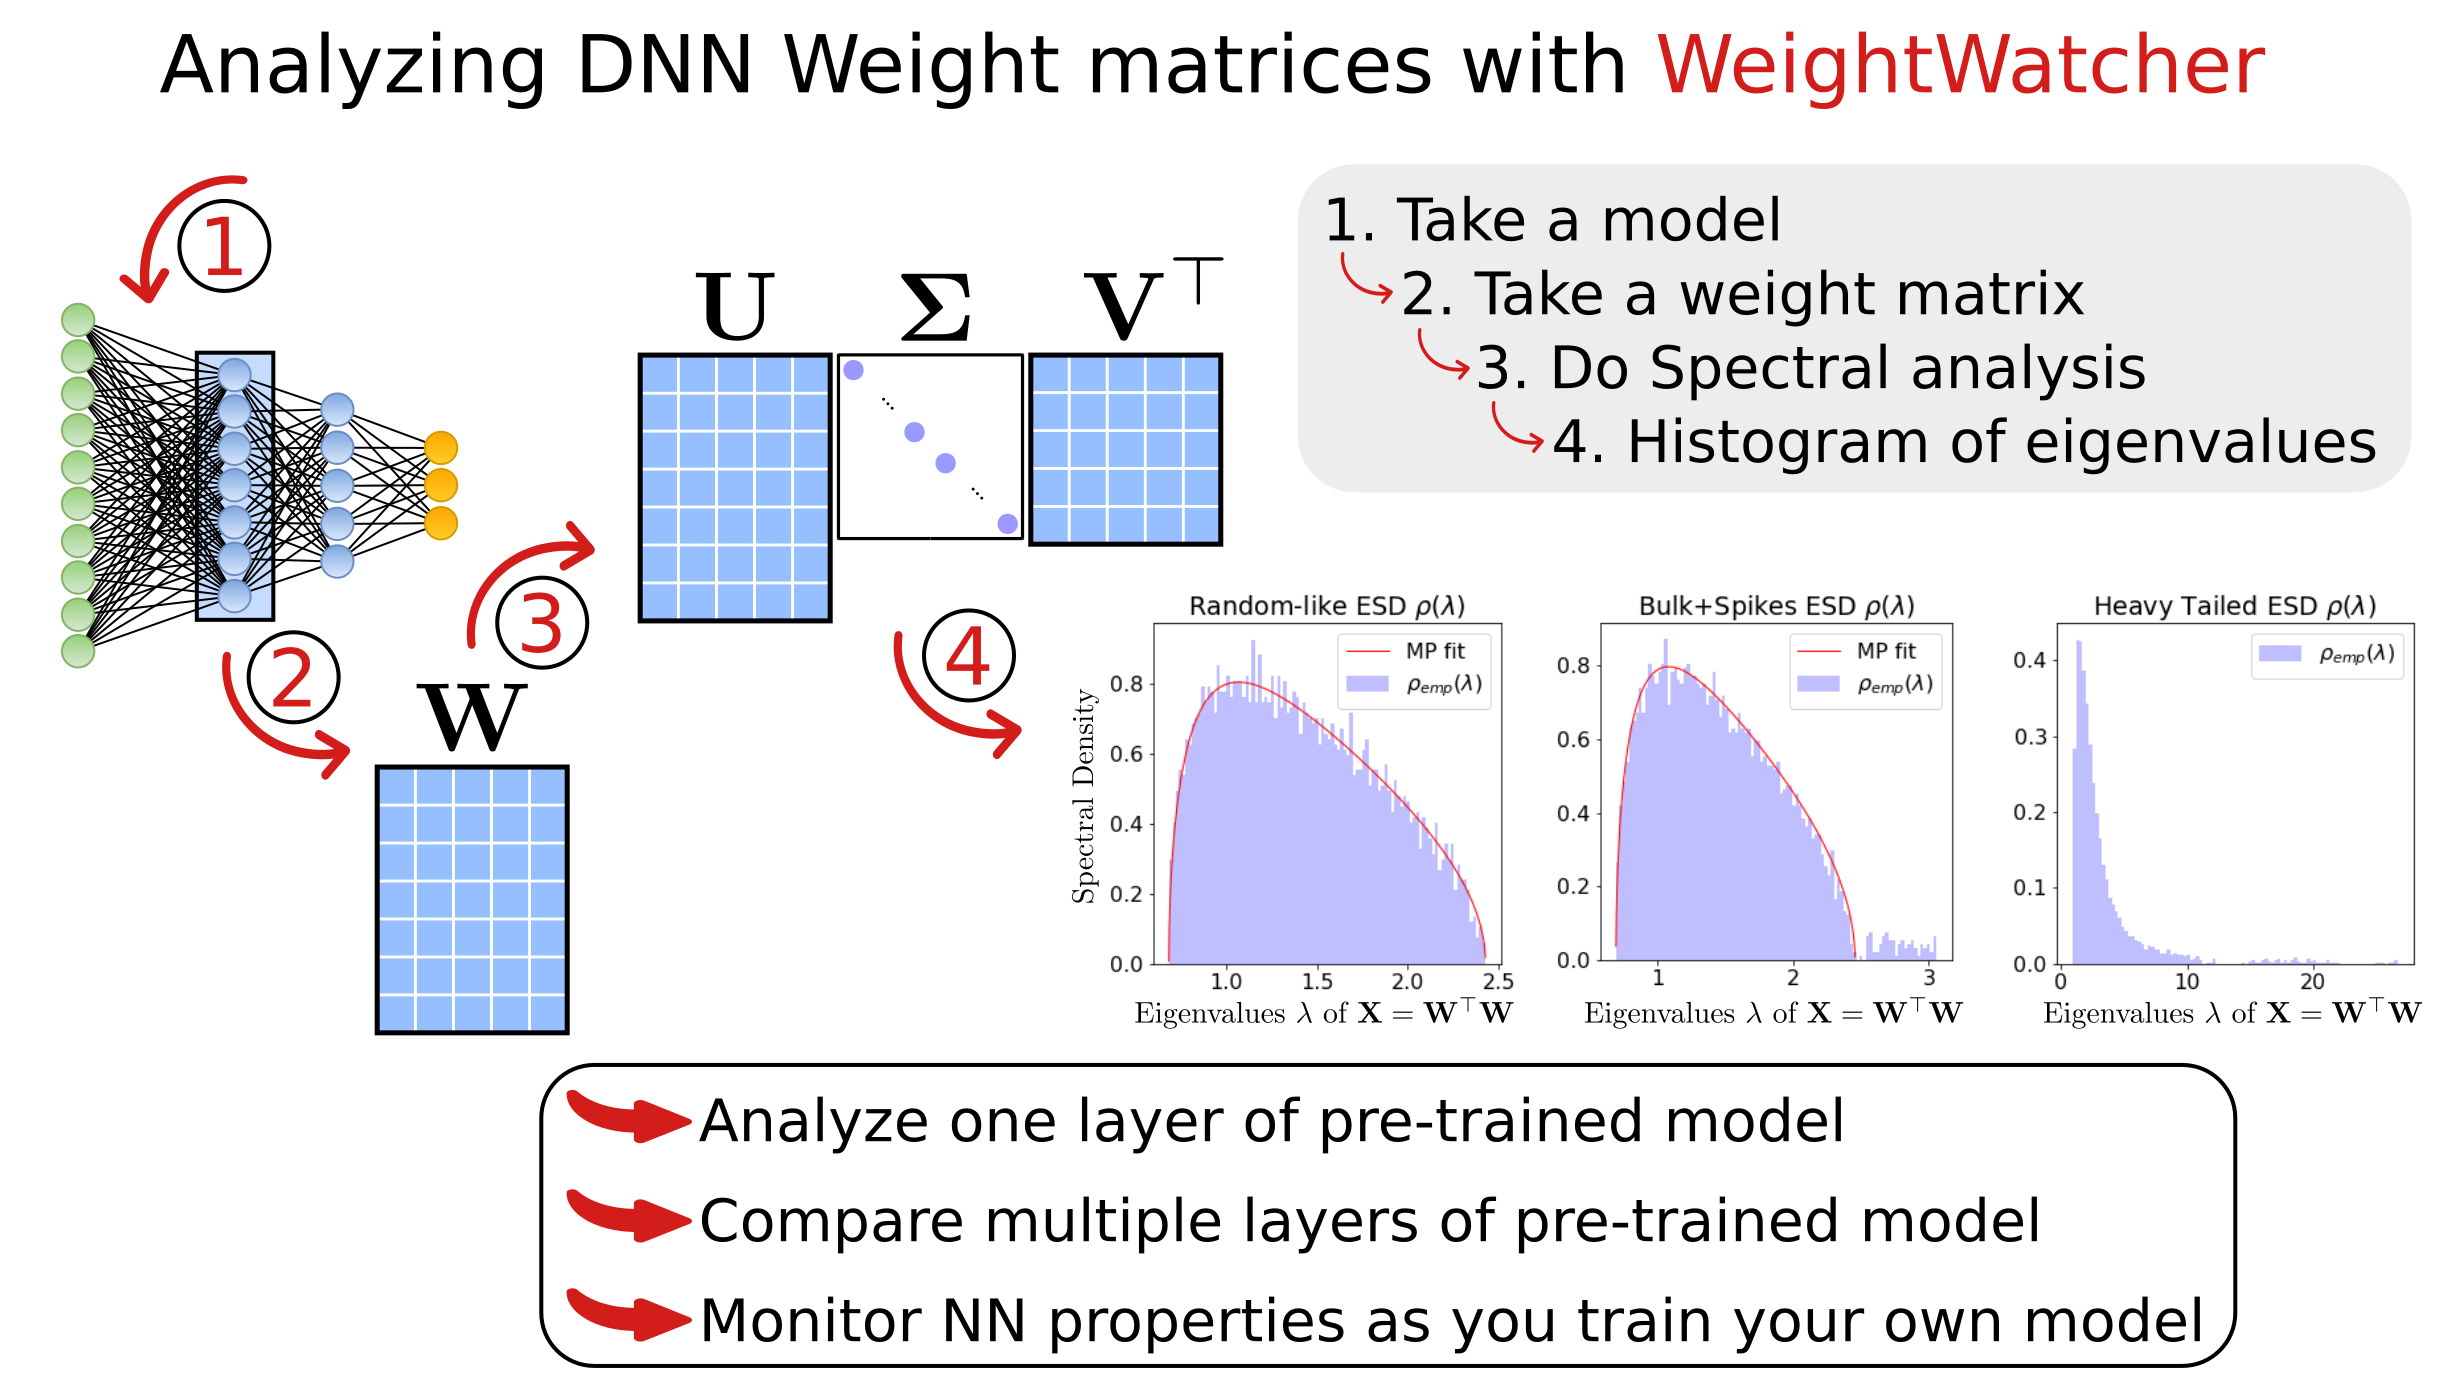
\includegraphics[width=15.0cm]{img/WeightWatcher_v2}
%    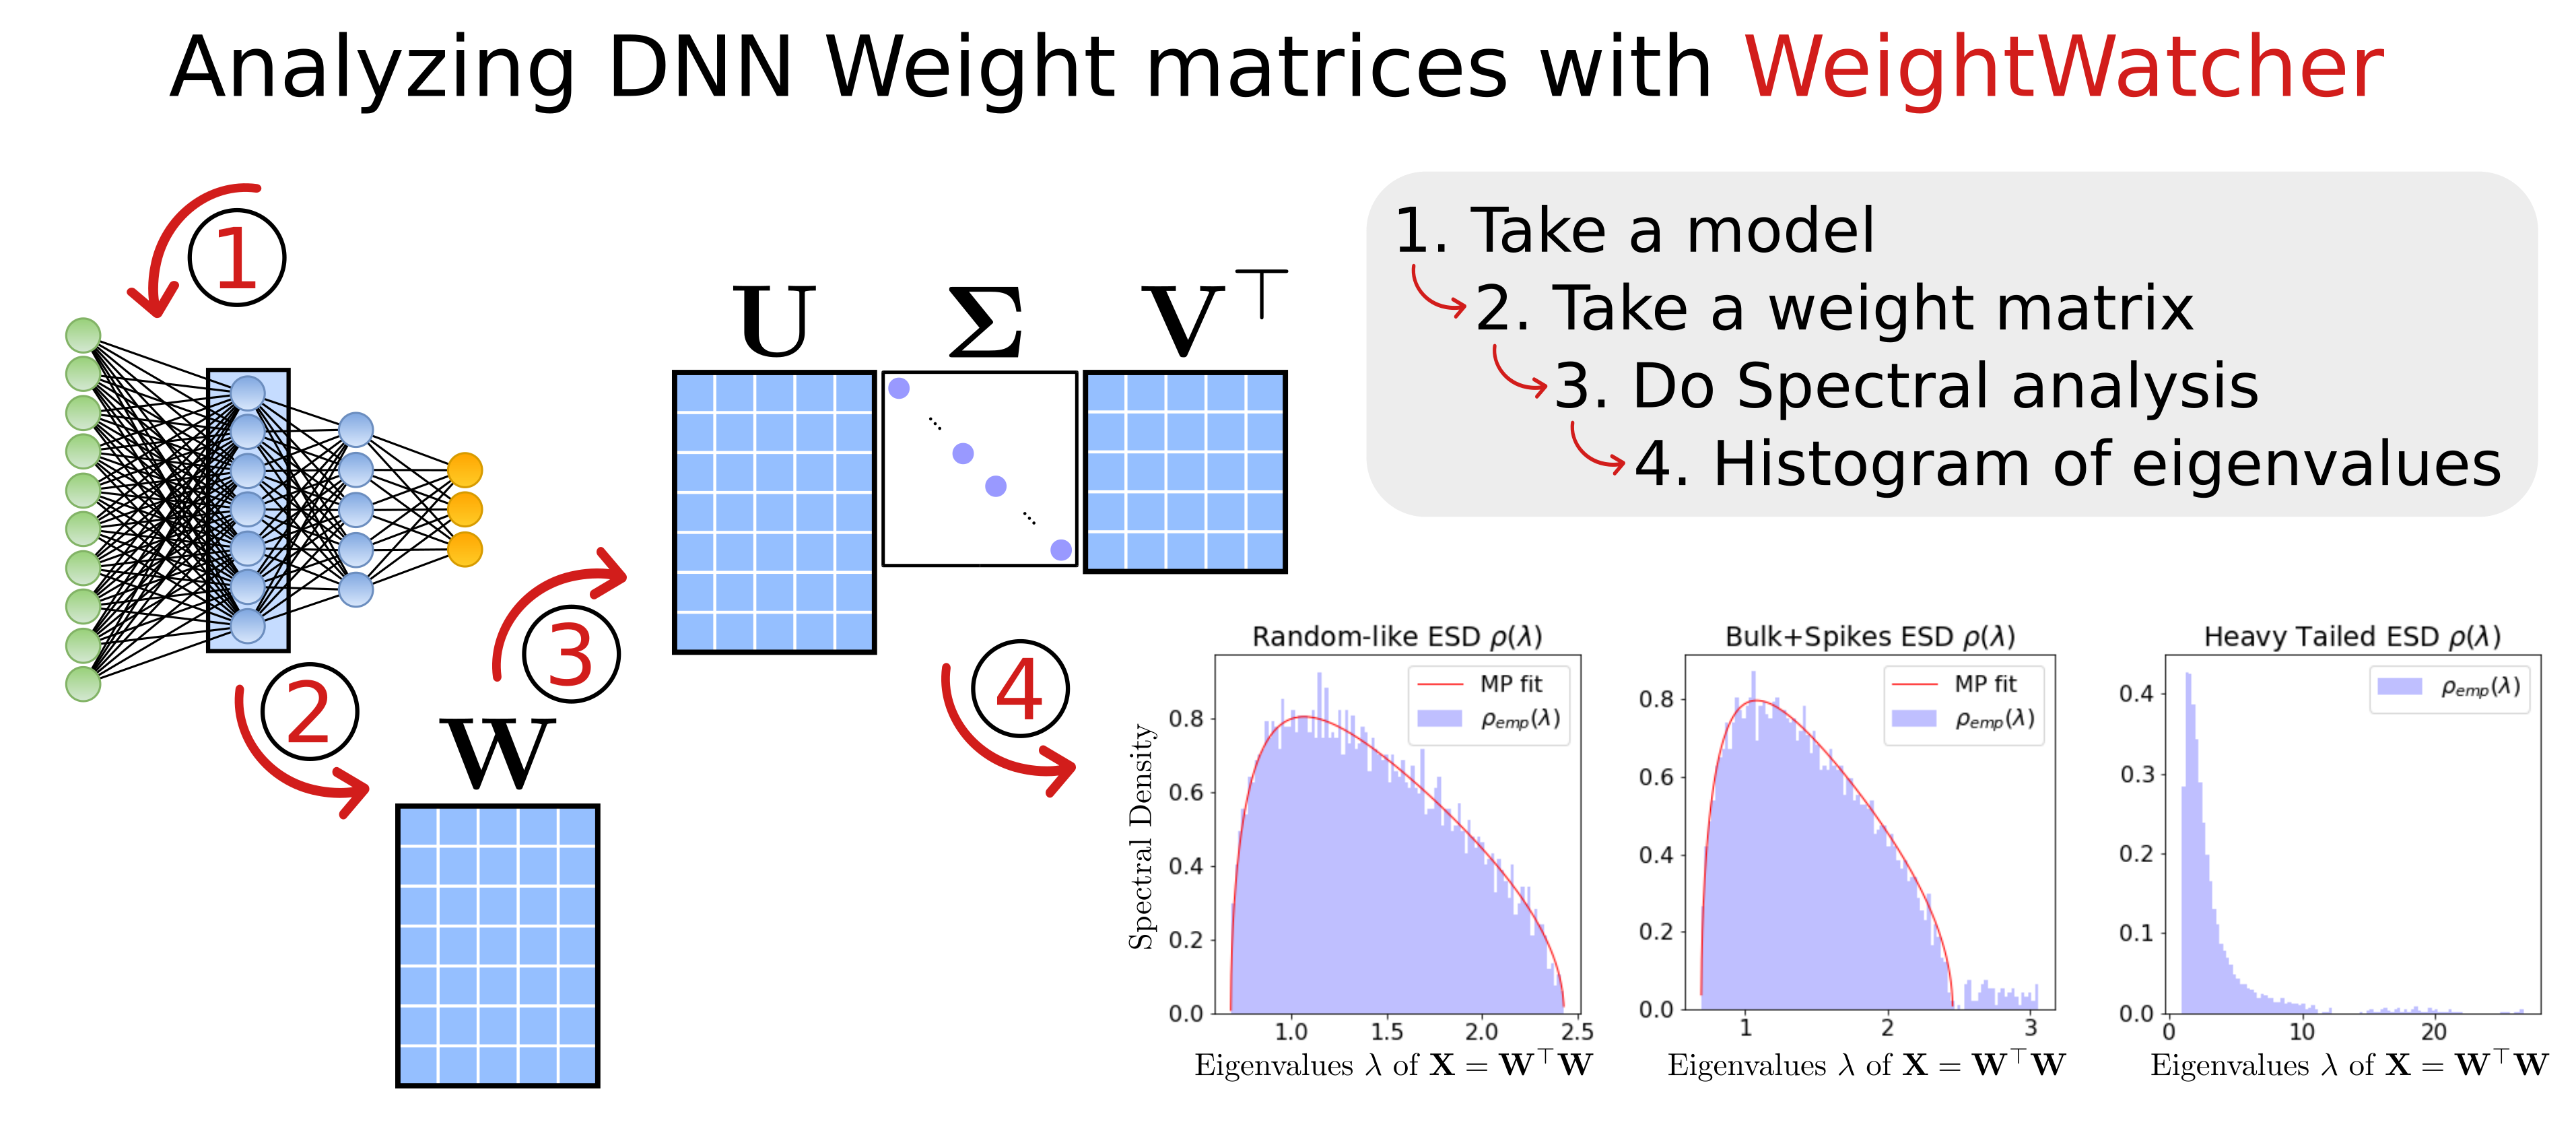
\includegraphics[width=15.0cm]{img/WeightWatcher_v3}
%    \caption{Schematic of analyzing DNN layer weight matrices $\mathbf{W}$.  
%             Given an individual layer weight matrix $\mathbf{W}$, from either a fully-connected layer or a convolutional layer, perform a Singular Value Decomposition (SVD) to obtain $\mathbf{W} = \mathbf{U} \mathbf{\Sigma} \mathbf{V}^{T}$, and examine the histogram of eigenvalues of $\mathbf{W}^{T}\mathbf{W}$.
%             Norm-based metrics and PL-based metrics (that depend on fitting the histogram of eigenvalues to a truncated PL) can be used to compare models.
%             For example, one can analyze one layer of a pre-trained model, compare multiple layers of a pre-trained model, make comparisons across model architectures, monitor neural network properties during training, etc. 
%}
%    \label{fig:ww}
%\end{figure}



To avoid confusion, let us clarify the relationship between $\alpha$ and $\hat{\alpha}$.  
We fit the ESD of the correlation matrix $\mathbf{X}$ to a truncated PL, parameterized by 2 values: the PL exponent $\alpha$, and the maximum eigenvalue $\lambda_{max}$.
The PL exponent $\alpha$ measures the amount of correlation in a DNN layer weight matrix $\mathbf{W}$. 
It is valid for $\lambda\le\lambda_{max}$, and it is scale-invariant, i.e., it does not depend on the normalization of $\mathbf{W}$ or $\mathbf{X}$.
The $\lambda_{max}$ is a measure of the size, or scale, of $\mathbf{W}$.
Multiplying each $\alpha$ by the corresponding $\log\lambda_{max}$ weighs ``bigger'' layers more, and averaging this product leads to a balanced, Weighted Alpha metric $\hat{\alpha}$ for the entire~DNN.
We will see that for well-trained CV and NLP models, $\hat{\alpha}$ performs quite well and as expected, but for CV and NLP models that are potentially-problematic or less well-trained, metrics that depend on the scale of the problem can perform anomalously.  
In these cases, separating $\hat{\alpha}$ into its two components, $\alpha$ and $\lambda_{max}$, and examining the distributions of each, can be helpful.



\section{Predicting Trends in the Quality of State-of-the-art Models}

XXX.  THIS IS A VERY PRACTICAL PROBLEM THAT OUR THEORETICAL APPROACH, STRONGLY COUPLED AND MOTIVATED BY EMPIRICAL PRACTICE, CAN SOLVE.

\cite{MM20a_trends_TR} is Charles: ``Predicting trends in the quality of state-of-the-art neural networks without access to training or testing data''

XXX.  ABSTRACT FROM \cite{MM20a_trends_TR}:
In many applications, one works with neural network models trained by someone else.
For such pretrained models, one may not have access to training data or test data.
Moreover, one may not know details about the model, e.g., the specifics of the training data, the loss function, the hyperparameter values, etc.
Given one or many pretrained models, it is a challenge to say anything about the expected performance or quality of the models.
Here, we address this challenge by providing a detailed meta-analysis of hundreds of publicly-available pretrained models.
We examine norm based capacity control metrics as well as power law based metrics from the recently-developed Theory of Heavy-Tailed Self Regularization.
We find that norm based metrics correlate well with reported test accuracies for well-trained models, but that they often cannot distinguish well-trained versus poorly-trained models.
We also find that power law based metrics can do much better---quantitatively better at discriminating among series of well-trained models with a given architecture; and qualitatively better at discriminating well-trained versus poorly-trained models.
These methods can be used to identify when a pretrained neural network has problems that cannot be detected simply by examining training/test accuracies.


XXX.  CITE ALSO BARTLETT AND POGGIO AS DOING SOMETHING LOOSELY SIMILAR, AND THE GOOGLE CONTEST AS DOING SOMETHING LOOSELY SIMILAR BUT DIFFERENT.

\cite{BFT17_TR} is Bartlett: ``Spectrally-normalized margin bounds for neural networks''

\cite{LMBx18_TR} is Poggio: ``A surprising linear relationship predicts test performance in deep networks''


\subsection{Introduction OF PREDICTING TRENDS PAPER}
\label{sxn:intro}

XXX.  THIS IS THE INTRO FROM THE PREDICTING TRENDS PAPER.

A common problem in machine learning (ML) 
is to evaluate the quality of a given model.
A popular way to accomplish this
is to train a model and then evaluate its training/testing error.
There are many problems with this approach.
The training/testing curves give very limited insight into the overall properties of the model; 
they do not take into account the (often large human and CPU/GPU) time for hyperparameter fiddling;
they typically do not correlate with other properties of interest such as robustness or fairness or interpretability; 
and so on.
A related problem, in particular in industrial-scale artificial intelligence (AI), arises when the model user is not the model developer.
Then, one may not have access to the training data or the testing data.
Instead, one may simply be given a model that has already been trained---a pretrained model---and need to use it as-is, or to fine-tune and/or compress it and then use it.

Na\"{\i}vely---but in our experience commonly, among ML practitioners and ML theorists---if one does not have access to training or testing data, then one can say absolutely nothing about the quality of a ML model.
This may be true in worst-case theory, but models are used in practice, and there is a need for a practical theory to guide that practice.
Moreover, if ML is to become an industrial process, then that process will become compartmentalized in order to scale: some groups will gather data, other groups will develop models, and other groups will use those models.
Users of models cannot be expected to know the precise details of how models were built, the specifics of data that were used to train the model, what was the loss function or hyperparameter values, how precisely the model was regularized,~etc.

Moreover, for many large scale, practical applications, there is no obvious way to define an ideal test metric. 
For example, models that generate fake text or conversational chatbots may use a proxy, like perplexity, as a test metric.
In the end, however, they really require human evaluation. 
Alternatively, models that cluster user profiles, which are widely used in areas such as marketing and advertising, are unsupervised and have no obvious labels for comparison and/or evaluation.
In these and other areas, ML objectives can be poor proxies for downstream goals.

Most importantly, in industry, one faces unique practical problems such as determining whether one has enough data for a given model. 
Indeed, high quality, labeled data can be very expensive to acquire, and this cost can make or break a project.
Methods that are developed and evaluated on any well-defined publicly-available corpus of data, no matter how large or diverse or interesting, are clearly not going to be well-suited to address problems such as this.
It is of great practical interest to have metrics to evaluate the quality of a trained model---in the absence of training/testing data and without any detailed knowledge of the training/testing process.  
There is a need for a practical theory for pretrained models which can predict how, when, and why such models can be expected to perform well or~poorly.

In the absence of training and testing data, obvious quantities to examine are the weight matrices of pretrained models, e.g., 
properties such as norms of weight matrices and/or parameters of Power Law (PL) fits of the eigenvalues of weight matrices.
Norm-based metrics have been used in traditional statistical learning theory to bound capacity and construct regularizers; and PL fits are based on statistical mechanics approaches to deep neural networks (DNNs).
While we use traditional norm-based and PL-based metrics, our goals are not the traditional goals.
Unlike more common ML approaches, we do not seek a bound on the generalization (e.g., by evaluating training/test errors), we do not seek a new regularizer, and we do not aim to evaluate a single model (e.g., as with hyperparameter optimization).
Instead, we want to examine different models across common architecture series, and we want to compare models between different architectures themselves.
In both cases, one can ask whether it is possible to predict trends in the quality of pretrained DNN models without access to training or testing data.  

To answer this question, we provide a detailed empirical analysis, evaluating quality metrics for pretrained DNN models, and we do so at scale.
Our approach may be viewed as a statistical meta-analysis of previously published work, where we consider a large suite of hundreds of publicly-available models, mostly from computer vision (CV) and natural language processing (NLP).
By now, there are many such state-of-the-art models that are publicly-available, e.g., 
hundreds of pretrained models in CV ($\ge 500$) and NLP ($\approx 100$).%
\footnote{When we began this work in 2018, there were fewer than tens of such models; now in 2020, there are hundreds of such models; and we expect that in a year or two there will be an order of magnitude or more of such models.}
For all these models, we have no access to training data or testing data, and we have no specific knowledge of the training/testing protocols. 
%
Here is a summary of our main results.
First, norm-based metrics do a reasonably good job at predicting quality trends in well-trained CV/NLP models.
Second, norm-based metrics may give spurious results when applied to poorly-trained models (e.g., models trained without enough data, etc.).
For example, they may exhibit what we call Scale Collapse for these models. 
Third, PL-based metrics can do much better at predicting quality trends in pretrained CV/NLP models.  
In particular, 
a weighted PL exponent (weighted by the log of the spectral norm of the corresponding layer) is 
quantitatively better at discriminating among a series of well-trained versus very-well-trained models
within a given architecture series; and
the (unweighted) average PL exponent is 
qualitatively better at discriminating well-trained versus poorly-trained models.
Fourth, PL-based metrics can also be used to characterize fine-scale model properties, including what we call layer-wise Correlation Flow, in well-trained and poorly-trained models; and they can be used to evaluate model enhancements (e.g., distillation, fine-tuning, etc.).
%
Our work provides a theoretically-principled empirical evaluation---by far the largest, most detailed, and most comprehensive to date---and the theory we apply was developed previously~\cite{MM18_TR, MM19_HTSR_ICML, MM20_SDM}.
Performing such a meta-analysis of previously-published work is common in certain areas, but it is quite rare in ML, where the emphasis is on developing better training protocols.



\section{A Simpson's Paradox---and the Need for Finer-scale Analysis}

XXX.  IF WANT A ONE SIZE FITS ALL METRIC, THEN CAN EXPECT A SIMPSONS PARADOX.  OUR TECHNIQUES CAN DIAGNOST THIS.  AND IN FACT WE SEE THAT.

\michael{Charles, put in a paragraph and the figure for the Simpson's paradox here.}

\charles{We apply our theory of Heavy Tailed Self-Regularization (HTSR) to predict the generalization accuracies of the pre-trained models provided in this contest, as a function of both model depth (L) and the solver hyperparameters (batch size, dropout, weight decay), and compare quality metrics that describe both the heavy-tailed shape and norm-based scale of the model layer weight matrices.  In doing so, we identify what amounts to a Simpson’s paradox, in which
shape and scale metrics show opposite behavior, and a combine metric resolves the paradox}



\begin{figure}[t!] 
    \centering
    \subfigure[Spectral Norm $\langle\log\Vert\mathbf{W}\Vert_{\infty}\rangle$]{
      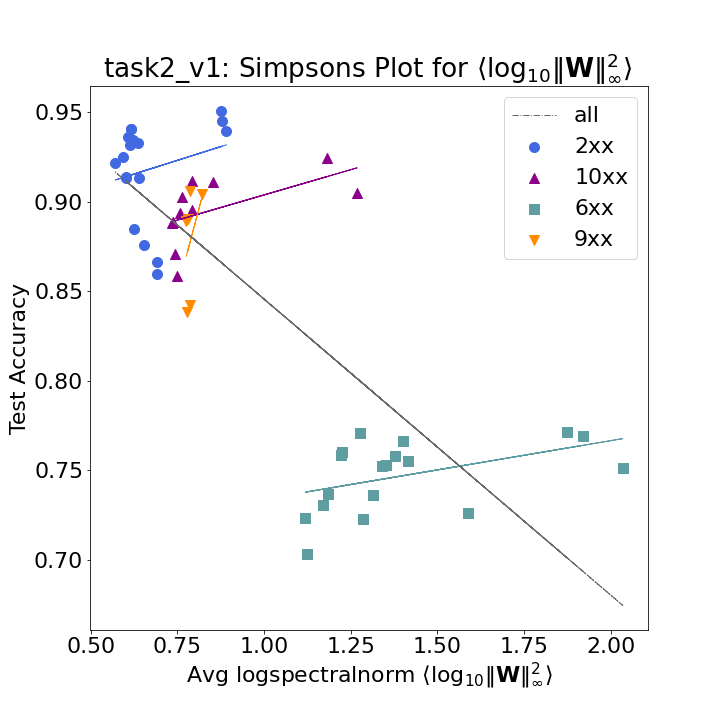
\includegraphics[width=4.0cm]{img/simpsons-task2-logspectralnorm.png}
    }
    \subfigure[Alpha Hat $\hat{\alpha}$]{
     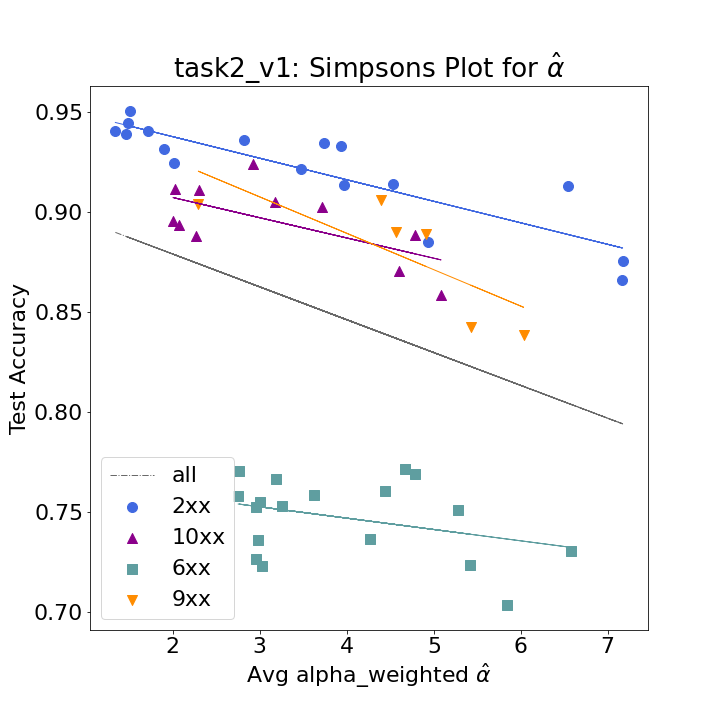
\includegraphics[width=4cm]{img/simpsons-task2-alpha_weighted.png}
    }
    \caption{Test accuracy as a function of the
Log Spectral Norm $\log\Vert\mathbf{W}\Vert_{\infty}$ 
and the HTSR Alpha Hat $\hat{\alpha}$ metrics
as model hyperparameters and depth are varied. 
Models from the NeurIPS Predicting Generalization contest.}
    \label{fig:simpsons}
\end{figure} 


\cite{JNBx19_fantastic_TR} is the terrible fantastic paper: ``Fantastic Generalization Measures and Where to Find Them''

\cite{JFYx20_contest_v10} is the contest: ``{NeurIPS} 2020 Competition: Predicting Generalization in Deep Learning (Version 1.0)''

\cite{BHO75} is Bickel: ``Sex Bias in Graduate Admissions: Data from Berkeley''




\section{Conclusion}

We have shown that weight matrix analysis derived from HT-SR Theory can be used to predict trends in the quality of state-of-the-art neural networks without access to training or testing data as well as identify Simpson's-like paradoxes in publicly-available NN models.
The HT-SR Theory underlying our analysis is quite different than theoretical approaches popular in ML, and indeed it is quite different than typical statistical mechanics approaches to NNs \cite{BKPx20}.
Recently, however, work motivated by HT-SR Theory has 
demonstrated that multiplicative noise in stochastic optimization leads to heavy tails~\cite{HodMah20A_TR,GSZ20_TR}; 
provided a random matrix analysis of random {F}ourier features, going beyond the {G}aussian kernel, to provide a precise phase transition and illustrate the corresponding double descent~\cite{ZCM20_TR}; 
provided exact expressions for double descent and implicit regularization via a notion of surrogate random design \cite{DLM19_Exact_TR}; 
demonstrated that good classifiers are abundant in the interpolating regime \cite{TKM20_TR};
shown how injecting noise into hidden states of recurrent NNs leads to implicit regularization~\cite{LEHM21_TR,Mah12}; and 
shown that analogous phase transitions hold for the {C}olumn {S}ubset {S}election and the {N}ystrom method~\cite{DKM20_TR}. 
We expect that the empirical results identified by tools from HT-SR Theory will provide guidance and constraints for future development of overparameterized machine learning models.


\bibliographystyle{icml2021}
\bibliography{dnns}


\end{document}


